% -*- mode: latex; -*- mustache tags:  
\documentclass[10pt,twoside,english]{_support/latex/sbabook/sbabook}
\let\wholebook=\relax

\usepackage{import}
\subimport{_support/latex/}{common.tex}

%=================================================================
% Debug packages for page layout and overfull lines
% Remove the showtrims document option before printing
\ifshowtrims
  \usepackage{showframe}
  \usepackage[color=magenta,width=5mm]{_support/latex/overcolored}
\fi


% =================================================================
\title{Learning Object-Oriented Programming, Design and TDD with Pharo}
\author{Stéphane Ducasse}
\series{The Pharo TextBook Collection}

\hypersetup{
  pdftitle = {Learning Object-Oriented Programming, Design and TDD with Pharo},
  pdfauthor = {Stéphane Ducasse},
  pdfkeywords = {Introduction, programming, design, testing, Pharo, Smalltalk}
}


% =================================================================
\begin{document}

% Title page and colophon on verso
\maketitle
\pagestyle{titlingpage}
\thispagestyle{titlingpage} % \pagestyle does not work on the first one…

\cleartoverso
{\small

  Copyright 2017 by Stéphane Ducasse.

  The contents of this book are protected under the Creative Commons
  Attribution-ShareAlike 3.0 Unported license.

  You are \textbf{free}:
  \begin{itemize}
  \item to \textbf{Share}: to copy, distribute and transmit the work,
  \item to \textbf{Remix}: to adapt the work,
  \end{itemize}

  Under the following conditions:
  \begin{description}
  \item[Attribution.] You must attribute the work in the manner specified by the
    author or licensor (but not in any way that suggests that they endorse you
    or your use of the work).
  \item[Share Alike.] If you alter, transform, or build upon this work, you may
    distribute the resulting work only under the same, similar or a compatible
    license.
  \end{description}

  For any reuse or distribution, you must make clear to others the
  license terms of this work. The best way to do this is with a link to
  this web page: \\
  \url{http://creativecommons.org/licenses/by-sa/3.0/}

  Any of the above conditions can be waived if you get permission from
  the copyright holder. Nothing in this license impairs or restricts the
  author's moral rights.

  \begin{center}
    
\includegraphics[width=0.2\textwidth]{_support/latex/sbabook/CreativeCommons-BY-SA.pdf}
  \end{center}

  Your fair dealing and other rights are in no way affected by the
  above. This is a human-readable summary of the Legal Code (the full
  license): \\
  \url{http://creativecommons.org/licenses/by-sa/3.0/legalcode}

  \vfill

  % Publication info would go here (publisher, ISBN, cover design…)
  Layout and typography based on the \textcode{sbabook} \LaTeX{} class by Damien
  Pollet.
}


\frontmatter
\pagestyle{plain}

\tableofcontents*
\clearpage\listoffigures

\mainmatter

\chapter{Implementing Joe the Box (to restart working on it when bloc is available for real)}\label{ch:joe}

\begin{figure}

\begin{center}
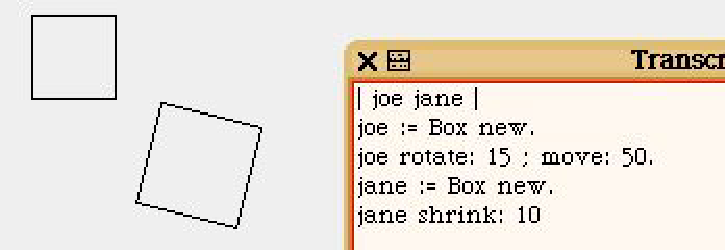
\includegraphics[width=0.8\textwidth]{/Users/ducasse/Workspace/FirstCircle/MyBooks/Bk-Writing/PharoBooks/LearningOOPWithPharoTrans/_result/pdf/Chapters/JoeTheBox/figures/joeTheBoxHeader.pdf}\caption{Playing with Joe the Box.\label{joeTheBox}}\end{center}
\end{figure}
 

Joe the Box is one the first example invented by A. Golderg (one of the inventor of object-oriented programming) to teach object-oriented programming. Joe the Box allows you the students to create box, shrink and rotate them. It is a simple system but it is really good to explain what classes, objects, messages (what to do) and methods (how to do) are.

In this chapter we will stress some key points about objects and class and you will program \textbf{Joe the Box}. For this you will implement the class \textcode{Box} (a class is a factory of objects its instances). Doing so you will learn how to describe behavior and state of
objects.  We start with a first implementation that we later refine. 
\section{Box's Behavior and State}
To create a Box, we ask an object called a class, here \textcode{Box} to create it by sending the message \textcode{new} to it.
The following expression create a box and its gets displayed on the screen. 

\begin{displaycode}{plain}
Box new 
\end{displaycode}

\begin{note}
To create an object we ask a class to create it using the message \textcode{new}.
\end{note}

\begin{note}
A class is a special kind of objects that act as a factory of objects.
\end{note}

A box has the following behavior: it knows how to draw itself, move to a given distance, move to a given point, rotate, grow and shrink.  A
typical scenario is described below. A graphical result is shown by the first figure of the chapter above.

\begin{displaycode}{plain}
| joe jane |
joe := Box new.
joe rotate: 15.
joe grow: 100.
joe move: 10 @ 10.
joe moveTo: 150 @ 200. 
jane := Box new.
jane move: 30 @ -30.
jane shrink: 40.
jane rotate: 45
\end{displaycode}

It is worth spending some time looking at this little program. First let us describe it.

\begin{itemize}
\item We defined two local variables \textcode{joe} and \textcode{jane}.
\item With the expression \textcode{Box new} we create a new instance of the class \textcode{Box}.
\item Then we assign this new instance to the variable \textcode{joe}.
\item Then we send the message \textcode{rotate:} to this object.
\item The object reacts to the message by modifying itself.
\item Then we send the message \textcode{grow:} to this object.
\item The object reacts to the message by modifying itself.
\end{itemize}

And we do the same for another instance of the class \textcode{ Box} that we assign to the variable \textcode{jane}.
\subsection{Instances are autonomous distinct entities}
In the script above we have two different objects: the box pointed by the variable \textcode{jane} and the one by the variable \textcode{joe}. 
In the following we will use \textcode{jane} and \textcode{joe} to represent the different boxes. In reality \textcode{jane} and \textcode{joe} are variables point to the boxes but it will make our explanations simpler to read and understand.  

\begin{itemize}
\item Each object is unique: box \textcode{jane} is not the same as box \textcode{joe}. 
\item Each object has its own state: box \textcode{jane} does not have the same size and tilt than box \textcode{joe}.
\item Objects of the same class understand the same message.
\item Objects of the same class exhibit the same behavior but they have their own properties.
\end{itemize}
\subsection{Messages: the What to do}
What you see is that we are telling the box to draw itself and a box to grow, shrink and rotate. From a Box programmer perspective, we do not know how the box move or rotate behavior is implemented. We just send \textbf{messages} to the objects and the objects react. Messages are orders sent to objects. Messages do not care how the order is defined.

\begin{displaycode}{plain}
joe grow: 10
\end{displaycode}

 When we send the \textcode{grow: 10} we expect the receiver of the message to change its size and we do not know how it is performed. 
 

\begin{note}
Messages are order sent to objects to tell them what to do (without taking care about how this order is defined and the precise steps required).
\end{note}
\subsection{Method: the How to do}
Later in this chapter you will define \textbf{methods} to define the behavior of Boxes (move, rotate:).
Methods are executed when an object receives a message. Methods describe precisely how a given message is implemented. A method will often change the state of an object and send other messages to the receiver and/or other objects. 

For example the following defined the method \textcode{grow:}.

\begin{displaycode}{plain}
grow: anInteger 
   "grow the receiver's size from anInteger"
   
    size := size + anInteger.
    self draw
\end{displaycode}

It is composed of

\begin{itemize}
\item A signature: here \textcode{grow: anInteger} indicates that we are defining the method \textcode{grow:} and that its argument is named \textcode{anInteger}.
\item A comment \textcode{\symbol{34}grow the receiver's size from anInteger\symbol{34}} which explains what the method is doing. 
\item A method body: here we increase the size of the receiver by changing its size value and we ask the receiver to redraw itself.
\end{itemize}
\subsection{About Behavior}
Before starting programming, we have to analyze the behavior of a box  to imagine a possible way to program it. Here is the 
behavior a box should have. A box should know how to:

\begin{itemize}
\item draw itself at a given location. When a new box is created it automatically displays itself. 
\item move to a given location (method \textcode{moveTo: aPoint}).
\item rotate from a given angle (method \textcode{rotate: anInteger}).
\item translate from a certain distance (method \textcode{move: aPoint}).
\end{itemize}

It is fundamental to start by looking at objects from their \textit{behavior}.  An object is a behavioral entity, i.e., an entity reacting to messages.  A similar behavior can be implemented by different manners so it is crucial not to start to think in terms of the internal structures that may represent the object but in
terms of the essence of the object, its \textit{behavior}.  
\subsection{From behavior to state}
Now from this description of the box's behavior, we should imagine a possible state for a box that could be used to implement the wished behavior.  As this example and the concept of box are familiar, we propose that box state is represented by a size, a position and a tilt.

In fact any box will be represented by such a triplet (size, position, and tilt) but each given object will have its own triplet values.  

For example, the box referenced by the variable \textcode{joe} in the script above has its \textit{own} state, i.e., its own size, position, and tilt.  

In the same way the box \textcode{jane} has a \textit{similar} state because it is also a box created from the class \textcode{Box} too but it has its own state which may or not equal to the one of \textcode{joe}.  

When the state of one given box changes it does not change the state of the other boxes.  This situation is illustrated by the first figure of this chapter.  
\subsection{About using anthropomorphic vocabulary}
Note the way we phrase the sentences describing box actions:  we do not say the box is displayed but it displays itself.  We always use
the active form where the subject is the object itself.  Considering the object as a living being is a good way to think in an object-oriented manner.  Imagine talking about an animal or a person you will say that the person acts and not is acted by others.  
\section{Defining the class Box}
To create a class we use a dedicated browser called the system browser
 or class browser.  To open such a browser, bring up the default menu and chose the menu item \textbf{open...} and the item \textbf{browser} (command-b).

To create a class, create first a new package (which represents a
group for all the classes we will create related to this small
project) by selecting the item \textbf{Add package} of the menu associated with the
leftmost pane of the browser. 

Name it for example \textbf{JoeTheBox}.  When you select the newly created package,
the system displays a template to help you defining a new class. 

\begin{displaycode}{plain}
Object subclass: #NameOfClass
   instanceVariableNames: 'instVarName1 instVarName2'
   classVariableNames: 'ClassVarName1 ClassVarName2'
   package: 'JoeTheBox'
\end{displaycode}


\begin{figure}

\begin{center}
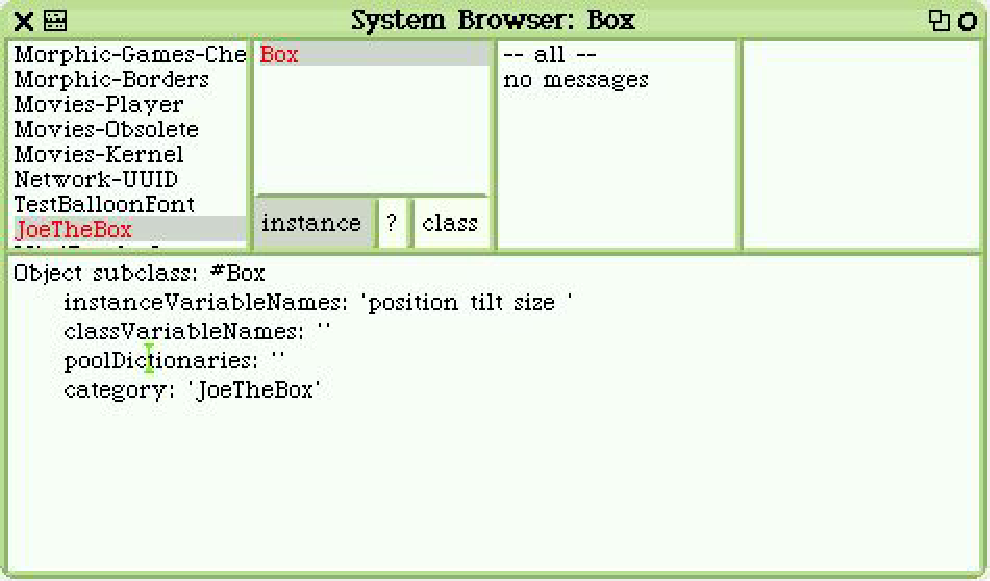
\includegraphics[width=0.8\textwidth]{/Users/ducasse/Workspace/FirstCircle/MyBooks/Bk-Writing/PharoBooks/LearningOOPWithPharoTrans/_result/pdf/Chapters/JoeTheBox/figures/classBoxCreated.pdf}\caption{The browser shows you that a new class has been created by displaying it in the second pane from the left.\label{classBoxCreated}}\end{center}
\end{figure}
 

Modify the proposed template to obtain the class definition and in the bottom pane bring the menu and choose the Accept menu item. 

\begin{displaycode}{plain}
Object subclass: #OBox
   instanceVariableNames: 'position size tilt '
   classVariableNames: ''
   package: 'Joe The Box'
\end{displaycode}

Now the class exists. The system shows you that the class is defined by displaying it in the second pane as shown in Figure\textasciitilde{}ref\{fig:classBoxCreated\}.  Using the terminology used in other programming languages we can say that the
class has been \textit{compiled}.  This means that we could already
create instances of this class, even if now this is not really useful
since they do not have any specific behavior.
	
\subsection{Explanation }
Here are some explanations about the class definition: 

\begin{itemize}
\item A box is a simple object. It does not refine the behavior of a class. Hence, it is a subclass \textcode{Object}.
\end{itemize}

\begin{itemize}
\item The internal state of box instances, such as the boxes \textcode{joe} and \textcode{jane}, is represented by instance variables of the class \textcode{Box}.  So line 2 we specify that the class \textcode{Box} has three instance variables by given their respective names.  Here the class \textcode{Box} has the instance variables \textcode{position}, \textcode{size}, and \textcode{tilt}.  This indicates to the class \textcode{Box} to create instances having three values representing the box's state. 
\end{itemize}

\begin{itemize}
\item We let empty the other parts of the templates because they are irrelevant for now.
\end{itemize}
\section{Important}
A class acts as an object factory, an instance model, or a mould. 
The instance variables describe the state that  the instances created 
by the classes will have. Each instance of the class will have the structure 
described by the class but filled with \textit{its own} values.

Instances have their own state but it follows the description given by the class. Two instances of the same class can have different values for the same instance variable but they cannot have a different number of instance variables. 

The \textit{factory} or mould metaphor is really useful to explain the difference between classes and instances. Here, the class \textcode{Box} describes and creates boxes of different size, position and tilt but all have these three characteristics.
\section{Initializing Instances}
Once the class is defined, create and inspect one of its instances by
executing scr:box or by using an inspector (see ch:usingInspector).  The
figure fig:uninitializedBox shows an inspector on a \textcode{Box}
instance.  All the instance variables have nil as
value.  Indeed, when an instance is created by invoking the method
new on a class, the default behavior of the
class is to return an uninitialized
instanceindex\{initialization\}.  Uninitialized means that all the
instance variables of the newly created instances have no value.  To
represent the emph\{no value\} concept, Smalltalk  uses the special object 
\textcode{nil} (Nil comes from the latin nihil which means
nothing.). 
That's why the instance variables of the inspected box have all as value \textcode{nil}.

\begin{displaycode}{plain}
Box new inspect
\end{displaycode}


\begin{figure}

\begin{center}
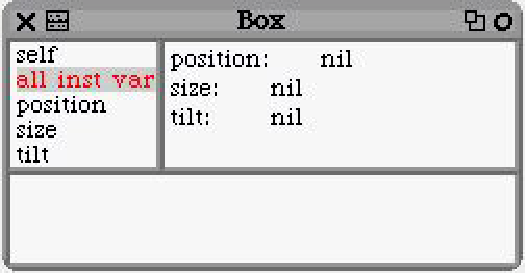
\includegraphics[width=0.8\textwidth]{/Users/ducasse/Workspace/FirstCircle/MyBooks/Bk-Writing/PharoBooks/LearningOOPWithPharoTrans/_result/pdf/Chapters/JoeTheBox/figures/unintializedBox.pdf}\caption{Inspecting a \textit{non initialized box}: all its instance variables \label{unintializedBox}}\end{center}
\end{figure}
 

Having uninitialized values is not really good because methods may not
work or have to test if the variables have been correctly initialized. 
But even then this is not satisfactory because if an instance variable
is not initialized it is difficult to know the value to initialize it. 
In fact the best solution is to initialize the instance as soon as it
is created.  

For that purpose we specialize the method \textcode{initialize} that sets up
a default state for a box.  The method \textcode{Box\textgreater{}\textgreater{}initialize} is
automatically invoked by the method \textcode{new} on newly created
instances.  This method sets the instance variables values.  Once this
method defined, in the bottom pane of the inspector evaluate the expression 
\textcode{self initialize}. If you closed the inspector or want to convince you that the method \textcode{initialize} is invoked when a new instance is created,  reuse scrref\{scr:box\} to check that the created
instance is now well initialized. In both cases, you should obtain a situation 
similar to the one described by the figure fig:initializedBox.

\begin{displaycode}{plain}
Box >> initialize
	"A box is initialized to be in the center of the screen, with 
	50 pixels size and 0 tilt"
	
	size := 50.
	tilt := 0.
	position := World bounds center
\end{displaycode}
\section{Accessing Instance Variables}
The method \textcode{initialize} above illustrates an important aspect of
the object model of Pharo. The instance variables are accessible from
the methods as if they were defined in the method body. For example, 
we are assigning \textcode{50} in the instance variable \textcode{size}. The instance 
variable \textcode{size} is accessible from any method of the class \textcode{Box}.

Contrary to the index\{local variables\}  of a
script  (\textcode{\textbar{} caro \textbar{}} for example) which do not exist after the script execution, instance
variables last the complete object life-time.  We propose you some
experiments to really understand this phenomena below.  Note that this
behavior is not new, we used it constantly with the turtle.  For
example, we changed the direction of the turtle using the method
ct\{north\} which was somehow changing the internal turtle state representing its direction, then later used the direction to perform some other actions.

We propose you to do some experiments to really understand this notion. 
Define the methods ct\{size\} (mthref\{mt:size\}) which returns the value 
of the instance variable ct\{size\} and ct\{size: anInteger\} 
(mthref\{mt:sizeAssign\}) which changes the value of 
the instance variable ct\{size\} to be the one specified as argument. Such a kind of methods are called emph\{accessor\} methods because they only get and set information in instance variables. 
The code ct\{\string^size\} returns the value of the instance variable size.

\begin{note}
To return a value, use the character \textcode{\string^} followed by the expression whose value has to be returned.
\end{note}

\begin{displaycode}{plain}
Box >> size
   ^ size
\end{displaycode}

\begin{displaycode}{plain}
Box >> size: anInteger
   size := anInteger
\end{displaycode}

Now execute the following script and use the menu item menu\{print it\} to get the results we present in  scrref\{scr:instanceVarLife\} using emph\{returns\}. If you have an inspector opened on a box instance, you can also execute the messages ct\{self size\}, ct\{self size: 10\} in the bottom left part of the inspector. Perform some other experiments to prove yourself that you understand.

\begin{displaycode}{plain}
| joe jane |
joe := Box new.
joe size. 
>>> 50
joe size: 10.
joe size. 
>>> 10
joe size: 20.
joe size. 
>>> 20
joe size: joe size + 5.
joe size. 
>>> 25
jane := Box new.
jane size. 
>>> 50
\end{displaycode}

Now that you understand better instance variables, you should notice that instance variables are private information of objects so creating emph\{accessor\} methods like the methodsct\{size\} and ct\{size:\} above that only access and return the value of an instance variable open the privacy of instances. We say that the break the encapsulation of the object data. We will discuss in charef\{cha:accessor\} the use of accessorsindex\{accessor\} methods.

In summary we have: 

\begin{note}
Instance variables are accessible to all the methods of a class.  Instance variables last the same life-time than the object to which they belong to.
\end{note}

\begin{note}
Instance variables cannot be accessed from outside of  an object. Instance variables are only accessible from the methods of  the class that define them.
\end{note}
\section{Drawing a Box and Other Operations}
Now that we initialize a newly created box using the method \textcode{initialize}, we are in position to define methods without been worried about the initialization of instance variables.  

During your experiments you may want to clear the screen.  Use the scrref\{scr:clearingScreen\} for that purpose.

\begin{displaycode}{plain}
World clearTurtleTrails
\end{displaycode}

paragraph\{Method ct\{draw\}.\} We define the method ct\{draw\} that uses a
turtle but we hide it as shown by mthref\{mt:draw\}.  We create a
method, put it at the right position of the box, set the direction of
the turtle to the tilt of the box, use the black color and then draw a
square of the box size.

\begin{displaycode}{plain}
Box >> draw
   "Draw the receiver position in black"
   "Box new initialize draw"
	
   | aTurtle |
   aTurtle := Turtle new hidden.
   aTurtle jumpAt: position.
   aTurtle turnRight: tilt.
   aTurtle penColor: Color black.
   4 timesRepeat: [aTurtle go: size. 
                  aTurtle turnLeft: 90]
\end{displaycode}

As soon as the method is defined and all the methods it calls exist, it is possible to invoke it.
Test the method by executing the code ct\{self draw\} into the bottom pane of an inspector in a similar way than shown in figure\textasciitilde{}ref\{fig:drawingBox\}, or by executing scrref\{scr:draw\}.

\begin{displaycode}{plain}
| joe  |
joe := Box new.
joe draw
\end{displaycode}
\subsection{Exercise.}
Up until now, creating a new box did not displayed it.  Change the method ct\{initialize\} so that any new box is automatically displayed.
\section{Method grow:}
 The method ct\{grow: anInteger\} makes the box growing of a certain size and redraw itself to reflect this size change.  Propose a definition and  use the inspector or dedicated scripts to tests your method. 

 {[}{[}{[}
Box \textgreater{}\textgreater{} grow: anInteger 
   \symbol{34}grow the receiver's size from increment\symbol{34}
   
    size := size + anInteger.
    self draw
{]}{]}{]}

We propose the definition\textasciitilde{}ref\{mth:grow\} for the method ct\{grow:\}.
However, try scrref\{scr:growProblem\} to see that we have a problem and 
propose a solution.

\begin{displaycode}{plain}
| joe |
joe := Box new.
joe grow: 20.

joe grow: 40
\end{displaycode}

The problem we have is that the turtle grows and redisplay itself  well, but it does not remove the previous box shape. To solve that 
problem we propose you to define a method named ct\{undraw\} which  is similar to the draw method except that it draw the box using a 
transparent color (mthref\{mt:undraw\}).

\begin{displaycode}{plain}
Box >> undraw
   "erase the receiver"
   
   | aTurtle |
   aTurtle := Turtle new hidden.
   aTurtle jumpAt: position.
   aTurtle turnRight: tilt.
   aTurtle penColor: Color transparent.
   4 timesRepeat: [ aTurtle go: size.
                  aTurtle turnLeft: 90 ]
\end{displaycode}

Now that the method ct\{undraw\} is defined, the method ct\{grow:\} should 
call it before anything else as shown by mthref\{mt:goodGrow\}.

\begin{displaycode}{plain}
Box >> grow: increment 
   "grow the receiver's size from increment"

   self undraw.
   size := size + increment.
   self draw
\end{displaycode}

To be able to execute the script we presented at the beginning of the chapter, implement the methods
begin\{itemize\}
item  ct\{move: aPoint\} which translate the box 
from a distance in x and y specified as a point. 
item ct\{moveAt: aPoint\} which move the box to the specified point.
item ct\{rotate: anInteger\} which rotates the box of a given angle. 
item ct\{grow: anInteger\} 
that make grow and shrink the receiver by a given factor.
end\{itemize\}

section\{Limiting Duplication\}label\{sec:\}
The methods ct\{draw\} (mthref\{mt:draw\}) and ct\{undraw\}
(mthref\{mt:undraw\}) are nearly the same except for the color of the
turtle.  This is not really good, since every times we will change one
method we will have to change the other and there is chance that we
forgot. Note that on this really simple example this is not really a
problem but we want to show you a good principle.

Propose a solution to this problem. The idea is that to avoid
duplication, the methods ct\{draw\} and ct\{undraw\} can call a third
method with the color of the pen as argument. We could named this
method ct\{drawWithColor:\}. Try to implement such a method before
reading the solution.

The ct\{drawWithColor: aColor\} (mthref\{mt:drawWithColor\}) shows a
possible implementation, it factors out the duplicated code. Now
change the methods ct\{draw\} and ct\{undraw\} to call this method with
the right argument.

begin\{method\} label\{mt:drawWithColor\}
Box\textgreater{}\textgreater{}drawWithColor: aColor 
   \symbol{34}Draw the receiver using a given color\symbol{34}
	
   \textbar{} aTurtle \textbar{}
   aTurtle := Turtle new hidden.
   aTurtle jumpAt: position.
   aTurtle turnRight: tilt.
   aTurtle penColor: textbf\{aColor\}.
   4 timesRepeat: {[}aTurtle go: size.
                  aTurtle turnLeft: 90{]}
end\{method\}

comment\{begin\{method\}
Box\textgreater{}\textgreater{}draw
   \symbol{34}draw the receiver in black\symbol{34}
   
   self drawWithColor: Color black
end\{method\}

begin\{method\}
Box\textgreater{}\textgreater{}undraw
   \symbol{34}erase the receiver\symbol{34}
   
    self drawWithColor: Color transparent
end\{method\}\}

In general we should avoid as much as possible to have duplicated
code.  This is not a problem to duplicate code for a small experiment.
However, if you want to keep the code always think that you should
create other method to share and reuse the duplicated code. Creating
one or several methods to factor the duplicated code is a good trick
to cure duplicated code.

cadre\{Avoid duplicated code. Refactor the duplicated code by calling 
a method representing the duplicated code.\}

section\{Looking at Alternate  Designs\}
We said that the implementation we proposed is one of the multiple
ways of implementing the behavior of the ct\{Box\} class. In this
section we want to look at other possible implementations.  First let
us analyze the current implementation.  The class ct\{Box\} has its own
state via the instance variables ct\{tilt\}, ct\{position\}, and
ct\{size\} then gives a part of its state to a turtle, its tilt and 
position.  The ct\{Box\} class uses the ct\{Turtle\} class to realize
its behavior.  This is a common practice where a class do not repeat
behavior but reuse the behavior of an existing class.

We used the class ct\{Turtle\} because it was familiar to us.  However,
another class, the class ct\{Pen\} could have been a possible candidate
too.  Look at the class ct\{Pen\} and change the method
ct\{drawWithColor:\} to use it instead of ct\{Turtle\}.  What is
important is that the interface proposed by the class ct\{Box\} should
not changed.  We are changing the internal implementation of the class
ct\{Box \}but this should not change its behavior.

Now if we look carefully we see that the turtle or the pen instance
are created every time the box is draw and undraw.  In addition the
state of the box is systematically copied to the turtle state then
lost because a turtle is recreated and the previous one is lost.  One
idea would be to use a turtle as representing part of the box state.
Indeed a turtle has also a position and a tilt.  

Define the class ct\{BoxT\} as shown below in
clsref\{cls:alternateBoxDefinition\} and reimplement some of the box's
methods to convince you that this is possible. This solution has the
advantages that less objects are created, less state is copied from
the box to the turtle and as drawbacks that the class ct\{Box\} is tied
with the class ct\{Turtle\}.

begin\{classdef\}label\{cls:alternateBoxDefinition\}
Object subclass: \#BoxT
   instanceVariableNames: 'size turtle'
   classVariableNames: \textit{
   poolDictionaries: }
   category: 'Joe The Box'
end\{classdef\}

To help you we show two methods, mthref\{mt:boxAlternateInitialize\} and 
mthref\{mt:alternateDrawWith\}, that are important. Try to do it by 
yourself first. Implement all the other methods. 

begin\{method\}label\{mt:boxAlternateInitialize\}
BoxT\textgreater{}\textgreater{}initialize
   \symbol{34}A box is initialized to be in the center of the screen, with 
   50 pixels size and 0 tilt\symbol{34}
   
   size := 50.
   turtle := Turtle new hidden.
   turtle jumpAt: World bounds center.
end\{method\}

begin\{method\}label\{mt:alternateDrawWith\}
BoxT\textgreater{}\textgreater{}drawWithColor: aColor 
   \symbol{34}Draw the receiver using a given color\symbol{34}
	
   turtle penColor: aColor.
   4 timesRepeat: {[}turtle go: size.
                  turtle turnLeft: 90{]}
end\{method\}

section\{What you should have learned\}
Blabla here...

ifxwholebookrelaxelse
end\{document\}fi



% lulu requires an empty page at the end. That's why I'm using
% \backmatter here.
\backmatter

% Index would go here
\bibliographystyle{abbrv}
\bibliography{others.bib}
\end{document}
